\documentclass[11pt]{article}
\usepackage[margin=1in]{geometry}
\usepackage{booktabs}
\usepackage{amsmath, amssymb}
\usepackage{enumitem}
\usepackage[compact]{titlesec}
\usepackage{parskip}
\usepackage{graphicx}
\usepackage{multirow}
\usepackage{float}

\title{Evaluation of Custom Embedding Model $g_1$}
\author{}
\date{}

\begin{document}
\maketitle
\vspace{-4em}

\section*{Overview}

We aim to fine-tune a CALE embedding model to better associate cryptic crossword
definitions with their correct answers. Our first custom model, $g_1$, was trained using triplet margin loss
($\alpha = 1.0$, $p = 2$, 3 epochs, lr $= 2 \times 10^{-5}$, batch size 32)
on 69,921 training triplets ($\tau_1$), each consisting of:

\begin{center}
\begin{tabular}{@{}lll@{}}
\textbf{Anchor} & $f_{\text{clue}}(\text{def}) $ & the definition word, embedded in its cryptic clue context \\
\textbf{Positive} & $f_{\text{wndef}}(\text{ans})$ & the correct answer, embedded with its WordNet definition \\
\textbf{Negative} & $f_{\text{wndef}}(\text{dist})$ & a distractor word, embedded with its WordNet definition \\
\end{tabular}
\end{center}

\noindent The training objective pushes the anchor closer to the positive and
farther from the negative. We evaluated $g_1$ on 46,506 held-out validation 
triplets using both the
training metric (L2 distance) and the research metric (cosine similarity). 

\subsection*{Data Leakage from Seen Vocabulary}

While every anchor (clue-contextualized definition) in the validation set is 
unseen, positives and negatives 
may appear in both the training and validation splits---an unavoidable feature 
of language reusing words. Where appropriate, we stratify analyses by \emph{seen} 
and \emph{unseen} vocabulary, and use the $f_{\text{wndef}}$ phrase construction
strategy for decontextualized meanings.

\subsection*{Metric Mismatch: A Non-Issue}

We trained $g_1$ with L2 distance but evaluated with cosine similarity.
L2 and cosine agree on every analysis in this evaluation---triplet accuracy,
margins, context effects, and stratified comparisons all produce the same
qualitative findings under both metrics.\footnote{This is expected when
embedding norms are tightly concentrated: L2 distance depends on both
direction and magnitude, while cosine depends only on direction, so the two
converge when magnitudes are similar. Under $g_1$, the \texttt{wndef} norm
distribution has a coefficient of variation of $\sim$3\% (std 0.86 on a mean
of 27.9), and \texttt{f\_clue} is even tighter at $\sim$2.6\%.} The choice
of training metric did not distort any of our conclusions, so below we report
metrics only in cosine similarity.

\section*{Task Performance and Overfitting}

The model clearly learned the triplet discrimination task: $g_1$ achieves
90.0\% triplet accuracy on held-out validation triplets, compared to
$g_\text{stock}$'s 38.8\%.\footnote{The fact that $g_\text{stock}$ scores
below chance (50\%) is itself informative: the $\tau_1$ distractors are
systematically more similar to the anchor than the true answers are under
pretrained $g_\text{stock}$. The training asked $g_1$ to invert this
ordering.} The \textit{margin}---the difference between the anchor-positive
similarity and the anchor-negative similarity for each triplet---tells us how
well-separated the correct answer is from the distractor. $g_1$'s validation
mean margin is 0.125, compared to $g_\text{stock}$'s $-0.054$. The negative
$g_\text{stock}$ margins confirm that distractors are typically more similar
to the anchor than answers are under the pretrained model.

\begin{figure}[H]
\centering
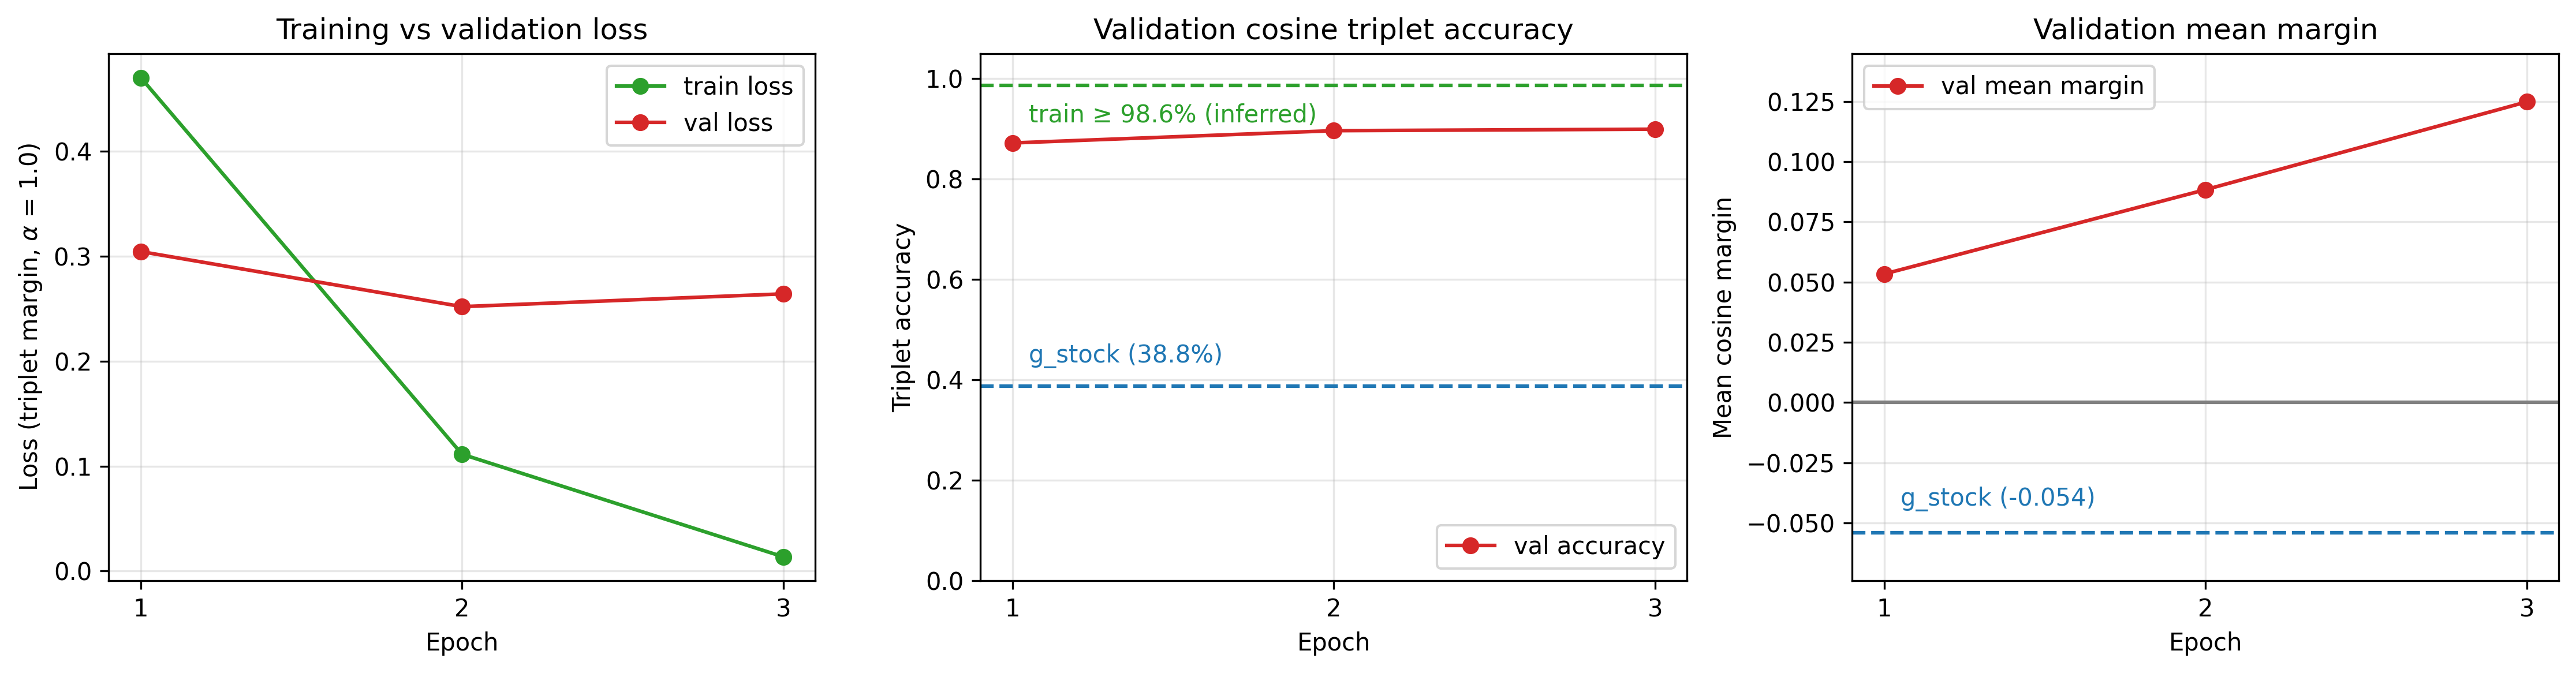
\includegraphics[width=\textwidth]{figures/g1be_training_dynamics.png}
\caption{\small Training dynamics across 3 epochs. Left: training loss (green)
diverges from validation loss (red) after epoch 2. Center: validation accuracy
plateaus near 90\%. Right: validation margins continue growing even as loss rises.}
\end{figure}

Training dynamics show classic overfitting: validation loss improved from epoch
1 to epoch 2 (0.305 $\to$ 0.252) but rose at epoch 3 (0.264), while training
loss fell to 0.014---a 19$\times$ train/val ratio. Notably, validation
accuracy barely changed from epoch 2 to 3 (89.7\% $\to$ 90.0\%) while
validation margins grew substantially (0.088 $\to$ 0.125). The model
polarized the validation set: triplets it already classified correctly were
pushed further apart, while the $\sim$10\% it got wrong incurred larger
penalties---which is why loss rose even as margins grew.

The gap between training accuracy ($\geq$98.6\% inferred from epoch
3 training loss) and validation
accuracy (90.0\%) confirms that $g_1$ performs better on data it trained on.
But this gap is modest, and stratifying the validation triplets by whether the
positive and negative words appeared in training tells us it didn't produce
word-level memorization:

\begin{figure}[H]
\centering
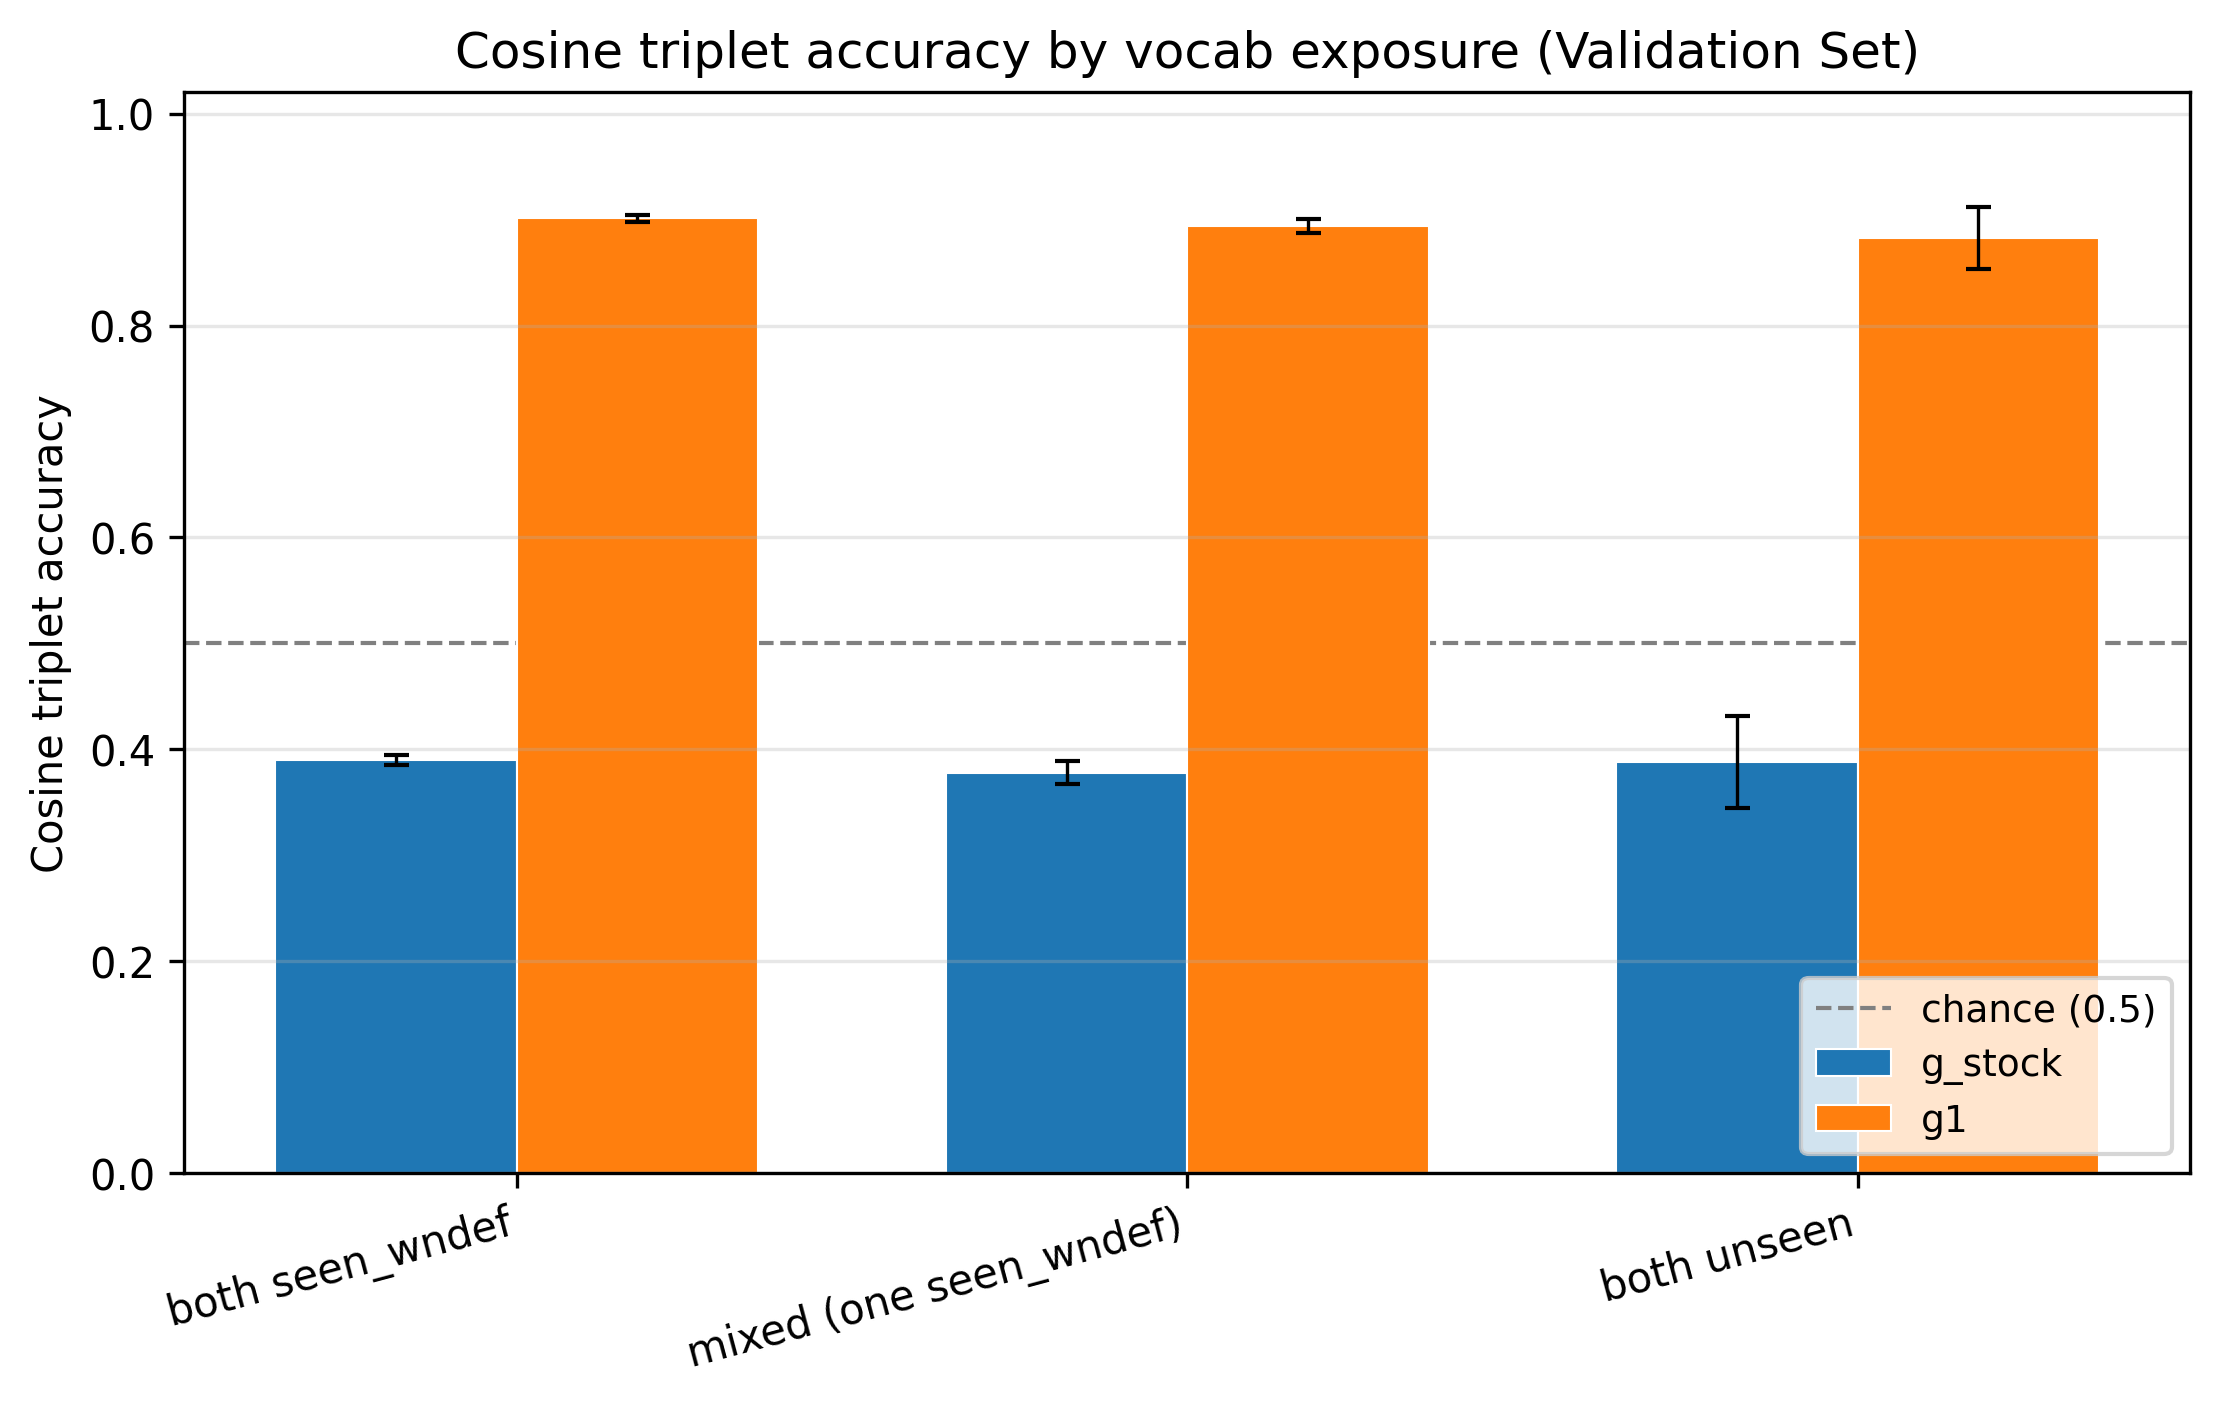
\includegraphics[width=0.85\textwidth]{figures/g1be_seen_unseen_cosine.png}
\caption{\small Cosine triplet accuracy by vocabulary exposure stratum, with
95\% confidence intervals. Both $g_\text{stock}$ and $g_1$ perform uniformly 
across strata. The original model is below chance (dashed line) in all three.}
\end{figure}

$g_1$'s performance is uniform across seen and unseen words; the overfitting
likely means we trained one epoch past optimal, but it didn't produce data
leakage at the word level.

\section*{Embedding Space: Compressed and Reorganized}

Fine-tuning contracted the embedding space substantially without collapsing it
dimensionally:

\begin{table}[h]
\centering
\begin{tabular}{llrrr}
\toprule
 & & $g_\text{stock}$ & $g_1$ & Shift \\
\midrule
\multirow{4}{*}{\texttt{wndef}}
 & Mean pairwise cosine & 0.412 & 0.561 & +0.149 \\
 & Total variance & 27.0M & 18.6M & $-31\%$ \\
 & Effective dimensionality & 41.1 & 45.4 & +4.4 \\
 & RSA $\rho$ & --- & 0.135 & --- \\
\midrule
\multirow{4}{*}{\texttt{f\_clue}}
 & Mean pairwise cosine & 0.317 & 0.452 & +0.135 \\
 & Total variance & 30.7M & 22.1M & $-28\%$ \\
 & Effective dimensionality & 52.3 & 103.2 & +50.8 \\
 & RSA $\rho$ & --- & 0.067 & --- \\
\bottomrule
\end{tabular}
\end{table}

The RSA measures whether words that were similar under $g_\text{stock}$ remain
similar under $g_1$. At $\rho = 0.14$ for \texttt{wndef} and $\rho = 0.07$ for
\texttt{f\_clue}, $g_1$ didn't refine the pretrained similarity
structure---it essentially discarded it and built something new. The pairwise
cosine increase (+0.15) means unrelated words became more similar to each
other, undermining discriminability.

Total variance decreased while effective dimensionality increased---especially
for \texttt{f\_clue}, where it nearly doubled (52 $\to$ 103). This means $g_1$
compressed the dominant directions of variation while spreading what remained
more evenly across dimensions. The space got smaller but flatter: it did not collapse, 
but it lost some of the structure of the original CALE model.

This compression is not localized to words the model trained on. Stratifying
the vocabulary by training exposure shows that seen and unseen words were
affected equally:

\begin{table}[h]
\centering
\begin{tabular}{lrr}
\toprule
& \multicolumn{2}{c}{Mean pairwise cosine} \\
\cmidrule(lr){2-3}
& $g_\text{stock}$ & $g_1$ \\
\midrule
Seen ($n = 36{,}082$) & 0.408 & 0.565 \\
Unseen ($n = 12{,}794$) & 0.431 & 0.557 \\
\bottomrule
\end{tabular}
\end{table}

The model applied a global transformation to the entire embedding space,
including regions it never directly optimized---a structural change to how
the model maps text to embedding space, not a local side effect of training
on specific words.

\section*{No Evidence of Cryptic Crossword Specific Learning}

The central question is whether $g_1$ learned to extract useful information
from cryptic clue context. $T\!=\!0$ measures decontextualized
definition--answer similarity (definition appears alone); $T\!=\!1$ measures
clue-contextualized definition--answer similarity (definition appears inside
its cryptic clue). The ATE is $\overline{T\!=\!1} -
\overline{T\!=\!0}$; a negative value means clue context pushed the definition 
farther from the answer.

\begin{figure}[H]
\centering
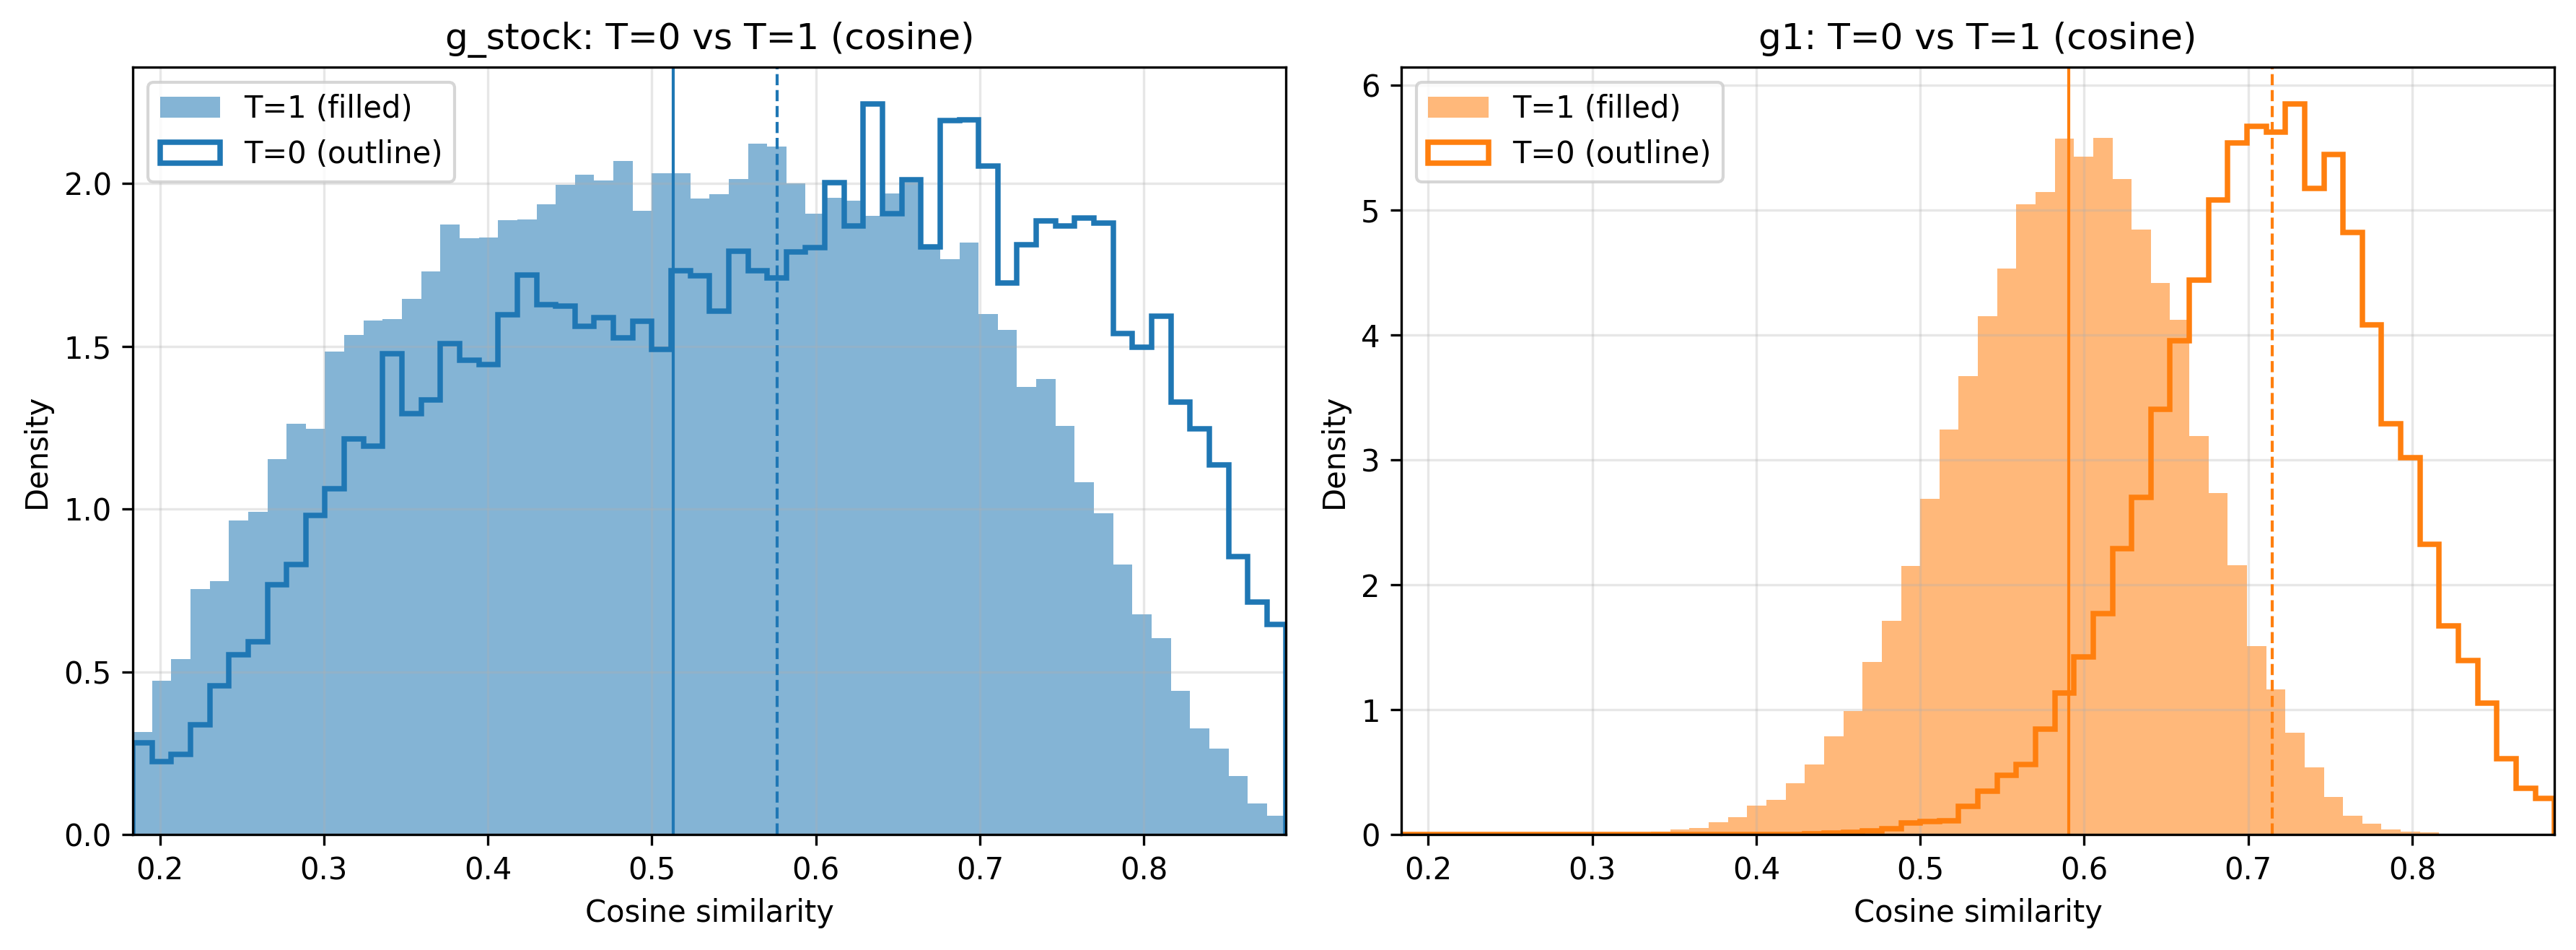
\includegraphics[width=\textwidth]{figures/g1be_t0_t1_cosine.png}
\caption{\small Cosine similarity distributions for $T\!=\!0$ (definition alone) and
$T\!=\!1$ (definition in clue context). Under $g_\text{stock}$ (left), the
distributions overlap substantially. Under $g_1$ (right), both distributions
tightened and shifted right, but $T\!=\!0$ shifted much more than $T\!=\!1$,
widening the gap between them.}
\end{figure}

\begin{table}[h]
\centering
\begin{tabular}{lrr}
\toprule
& $g_\text{stock}$ & $g_1$ \\
\midrule
$T\!=\!0$ (definition alone) & 0.576 & 0.715 \\
$T\!=\!1$ (definition in clue) & 0.513 & 0.591 \\
ATE ($T\!=\!1 - T\!=\!0$) & $-0.063$ & $-0.124$ \\
\% pairs where context hurts & 71.3\% & 93.4\% \\
\bottomrule
\end{tabular}
\end{table}

Under $g_1$, decontextualized definition-answer pairs became closer together 
($\Delta T\!=\!0$: +0.139), as did the clue-contextualized definition-answer pairs but 
to a much lesser extent ($\Delta T\!=\!1$: +0.078). The ATE doubled in magnitude, and the
fraction of pairs where context is misleading rose from 71\% to 93\%.

The custom model did not learn to exploit cryptic clue structure. Under $g_1$, 
clue context became even more misleading.

\section*{Summary}

Customizing the model fundamentally reorganized the
embedding space, made random words more similar to each other, and amplified
rather than reduced the misdirection from clue context. The next set of investigations 
will test which methodological issues---distractor design, phrase
format, noun bias, sense selection---contributed to this behavior.

\end{document}
